\documentclass[tikz,border=10pt]{standalone}
\usetikzlibrary{trees}

\begin{document}

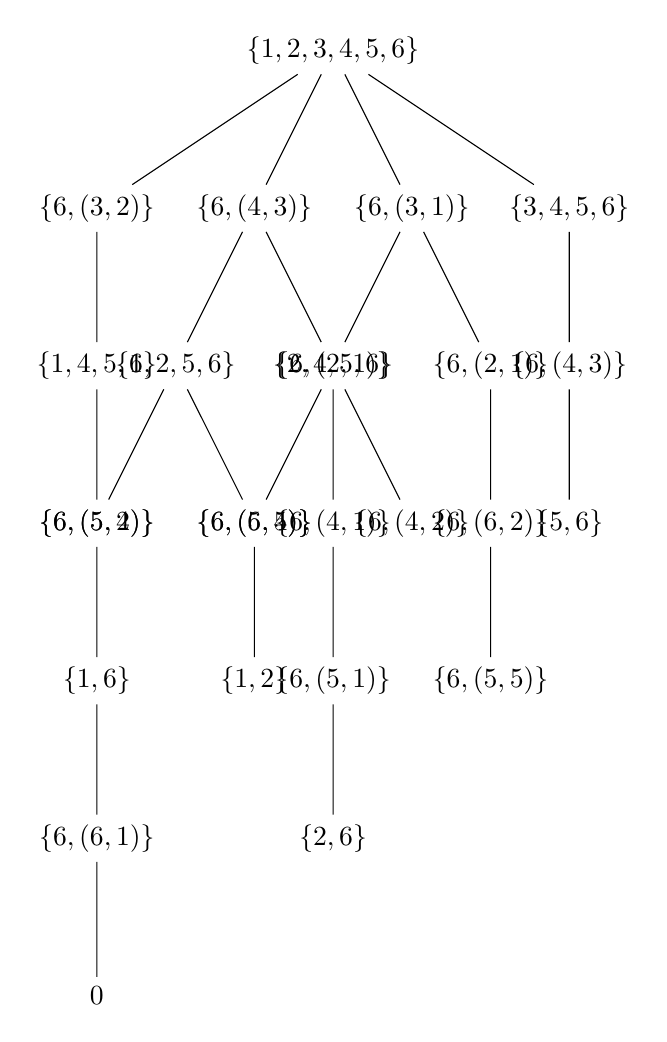
\begin{tikzpicture}[grow=down, level distance=2cm,
  sibling distance=2cm, every node/.style={align=center}]
  
  % Define the root node
  \node {$\{1, 2, 3, 4, 5, 6\}$}
    child {node {$\{6, (3, 2)\}$}
      child {node {$\{1, 4, 5, 6\}$}
        child {node {$\{6, (5, 4)\}$}
          child {node {$\{1, 6\}$}
            child {node {$\{6, (6, 1)\}$}
              child {node {$0$}}
            }
          }
        }
      }
    }
    child {node {$\{6, (4, 3)\}$}
      child {node {$\{1, 2, 5, 6\}$}
        child {node {$\{6, (5, 2)\}$}}
        child {node {$\{6, (6, 5)\}$}
          child {node {$\{1, 2\}$}}
        }
      }
      child {node {$\{6, (2, 1)\}$}
        child {node {$\{6, (4, 1)\}$}
          child {node {$\{6, (5, 1)\}$}
            child {node {$\{2, 6\}$}}
          }
        }
      }
    }
    child {node {$\{6, (3, 1)\}$}
      child {node {$\{2, 4, 5, 6\}$}
        child {node {$\{6, (5, 4)\}$}}
        child {node {$\{6, (4, 2)\}$}}
      }
      child {node {$\{6, (2, 1)\}$}
        child {node {$\{6, (6, 2)\}$}
          child {node {$\{6, (5, 5)\}$}}
        }
      }
    }
    child {node {$\{3, 4, 5, 6\}$}
      child {node {$\{6, (4, 3)\}$}
        child {node {$\{5, 6\}$}}
      }
    };
  
\end{tikzpicture}

\end{document}